\documentclass{beamer}
\usepackage{animate}
\usepackage{multimedia}
\usepackage[english,russian]{babel}

\usepackage{pgfpages}
\setbeameroption{show notes on second screen}
%https://tug.ctan.org/macros/latex/contrib/beamer/doc/beameruserguide.pdf

\usepackage[T2A]{fontenc}
\usepackage[utf8]{inputenc}

\setbeamertemplate{caption}[numbered]

\usetheme{CambridgeUS}
\usecolortheme{dolphin}


\title[Графический конвейер]{Графический конвейер трехмерного преобразования}
\author[Быковских Д.А.]{Быковских Дмитрий Александрович}
\date{30.09.2023}

\begin{document}
	\begin{frame}
		\titlepage
	\end{frame}
	
	\begin{frame}{Упрощенная модель графического конвейера}{Shaders}
		\begin{columns}
			\begin{column}{0.5\textwidth}
				\begin{figure} 
					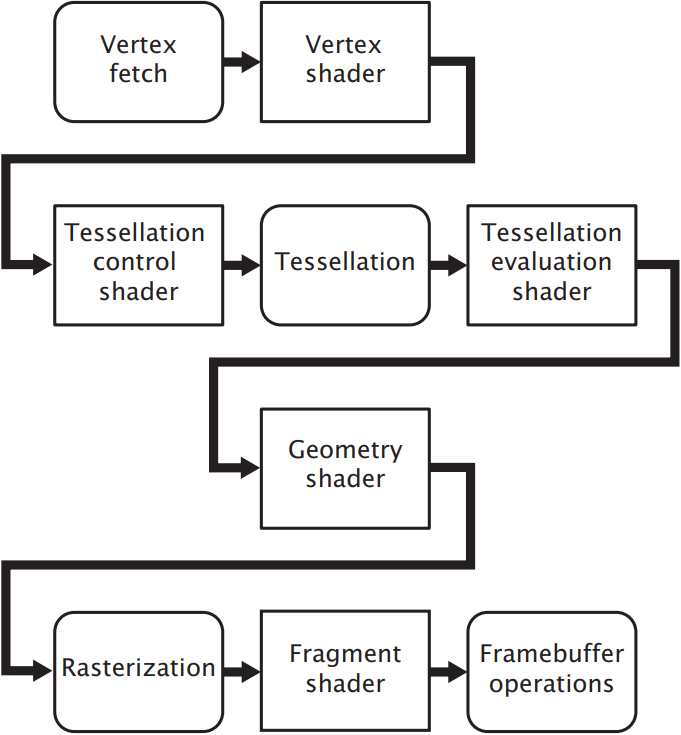
\includegraphics[width=0.9\textwidth]{images/Simplified_model_of_the_graphics_pipeline.png}
					\caption {Порядок вычисления шейдеров}
				\end{figure}
			\end{column}
			\begin{column}{0.5\textwidth}
				
				{\footnotesize
				
				Загрузка данных
				
				{\hfill Вершина (vertices)}
				
				\textbf{Вершинный шейдер}
				
				{\hfill Группа вершин (primitives/patches)}
				
				\textbf{Шейдер управление тесселяцией}
				
				Тесселяция
				
				\textbf{Шейдер определяющий тесселяции}
				
				{\hfill Примитивы (primitives)}
				
				\textbf{Геометрический шейдер}
				
				{\hfill Примитивы (primitives)}
				
				Растеризация и интерполяция
				
				{\hfill Пиксели (fragments)}
				
				\textbf{Пиксельный (фрагментный) шейдер}
				
				{\hfill Пиксели (fragments)}
				
				Операции с буферами кадров
				
				{\hfill Пиксели (Pixels)}
			}
			\end{column}
		\end{columns}
	\end{frame}
	
	\begin{frame}{Процесс построения изображения}
		\begin{figure} 
			\href{https://learnopengl.com/Getting-started/Coordinate-Systems}{
				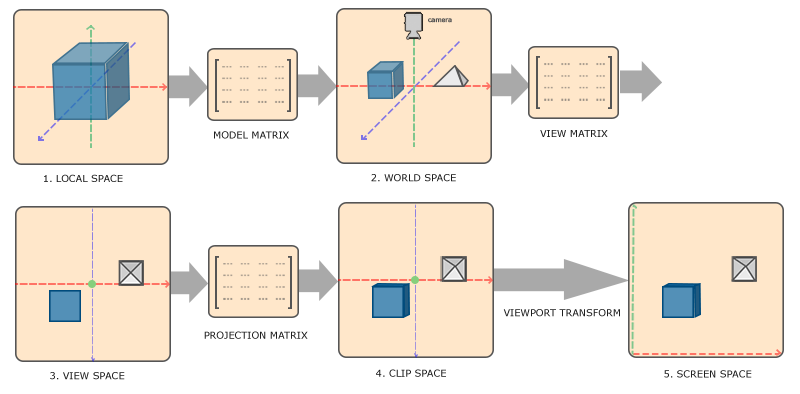
\includegraphics[width=\textwidth]{images/coordinate_systems.png}}
			\caption{Виды преобразований и системы координат}
		\end{figure}
		
	\note{
		{\hfill
		Модельные координаты (МК)
		}
		
		Преобразование моделирования
		
		{\hfill
		Внешние координаты (ВК)
		}

		Преобразование наблюдения

		{\hfill
		Координаты наблюдения (КН)
		}

		Преобразование проектирования
		
		{\hfill
		Координаты проекции (КП)
		}
		
		Преобразование нормировки и отсечение
		
		{\hfill
		Нормированные координаты (НК)
		}

		Преобразование поля просмотра
		
		{\hfill
		Координаты устройства (КУ)
		}
	}
	\end{frame}

	\begin{frame}{Процесс построения изображения}
		\begin{figure} 
			\href{https://www.researchgate.net/figure/Outline-of-the-graphics-pipeline_fig1_281810652}{
				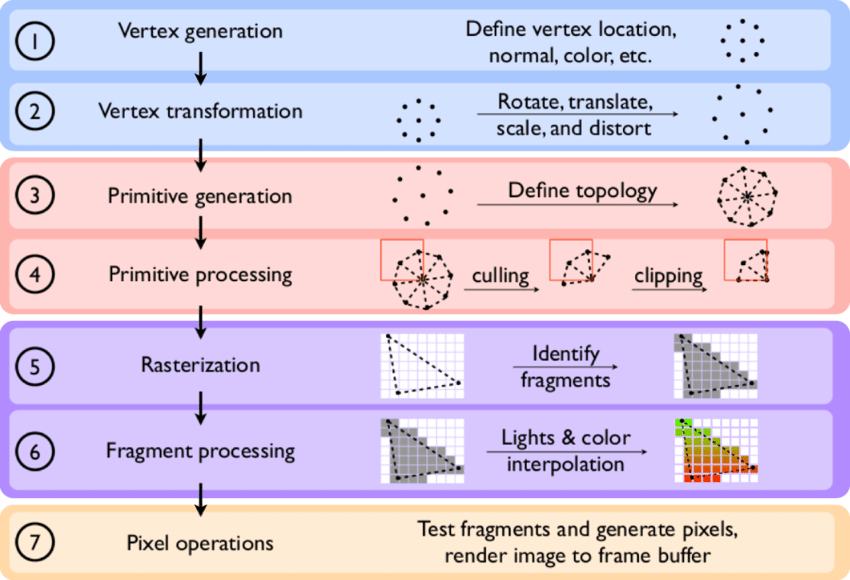
\includegraphics[width=0.75\textwidth]{images/Outline-of-the-graphics-pipeline.png}}
			\caption{Схема графического конвейера}
		\end{figure}
	\end{frame}
\end{document}